\chapter{Materials and methods}
In this chapter we will describe the steps of work performed in this project.
We will start with presentation of data which were available to us and which we used.
Then we will describe how we processed them to the form suitable as input for our neural network.
Finally we will show how we designed our neural network in detail and how we tested the performance of our designs.

\section{The pipeline}
Each step of our analysis was recorded in main analysis file named Snakefile.
This file is executable using Snakemake workflow engine.
The main reason to use this workflow management system was to make our analysis reproducible.
Snakemake also increases readability of the procedure and make orientation in the scripts easier.
Snakefile consists of rules, which define necessary input, output and the code needed to execute to get output from the input.
These rules can be visualized as directed acyclic graph symbolising the order of execution.
In the Figure \ref{fig:dag} we provide simplified graph containing all the rules and their dependencies.

\begin{figure}
    \centering
    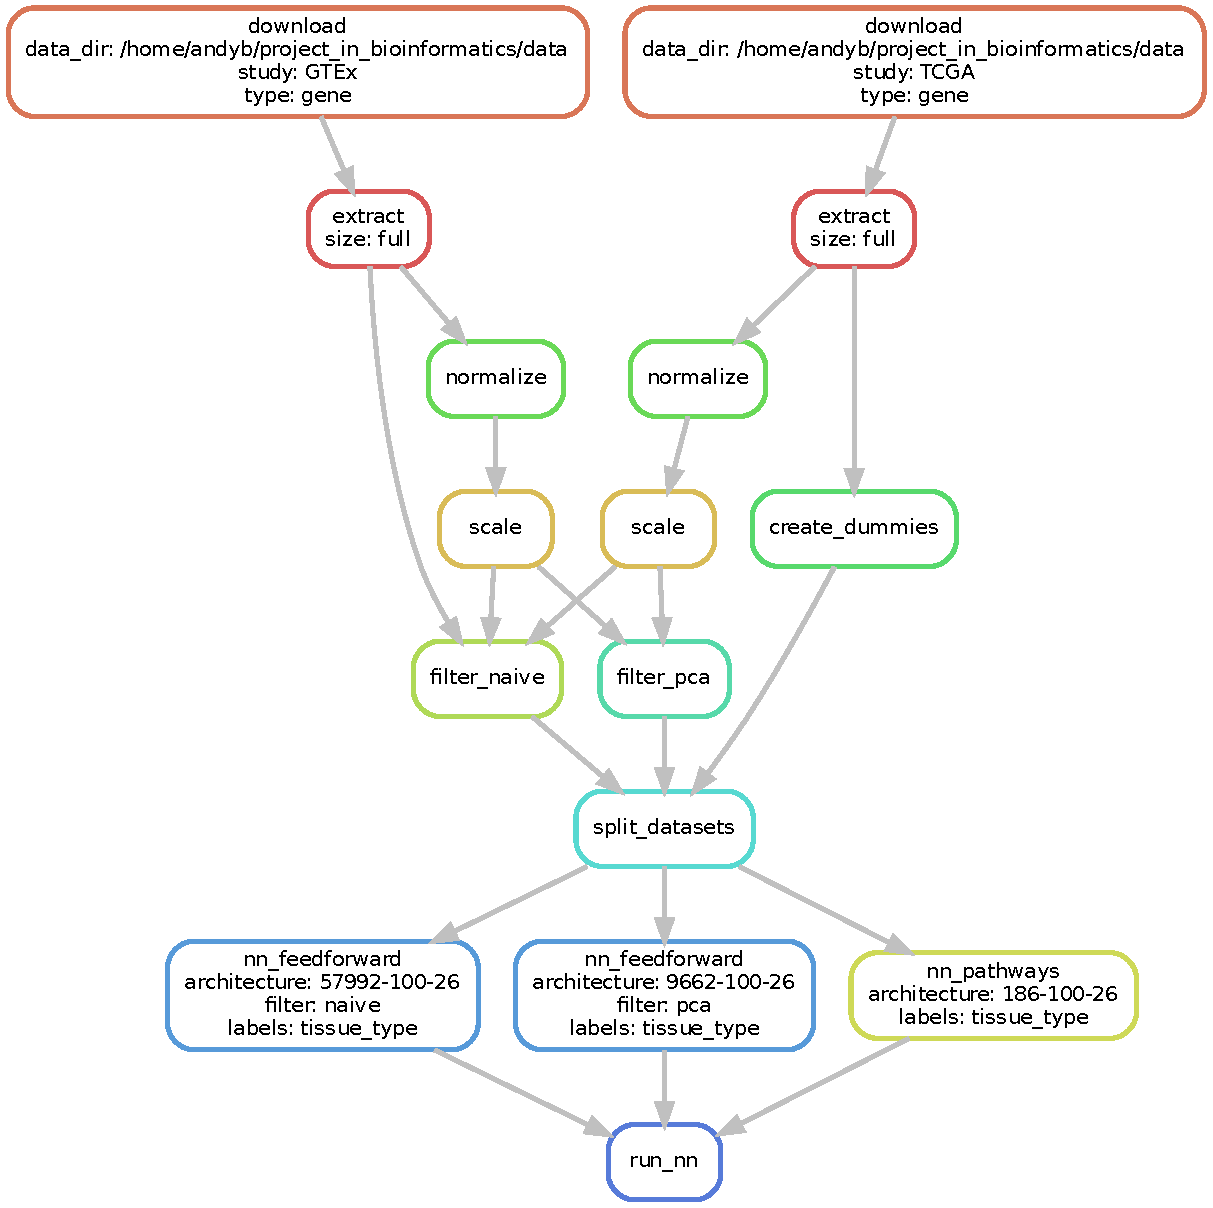
\includegraphics[width=\linewidth]{images/dag.pdf}
    \caption{Pipeline overview}
    \label{fig:dag}
\end{figure}

\section{Data available}
The main data which we worked with consisted of RNA-seq gene counts.
RNA sequencing has become a standard in studying a gene expression mainly due to its ability to detect transcriptional activity even without previously defined gene sequence. \cite{nellore2016rail}
A common use of this method is to determine expression level across the samples and then use this information to identify the patterns associated with outcome of interest.
In our project, we used expression data from two distinct sources, The Genotype-Tissue Expression project (GTEx) and The Cancer Genome Atlas (TCGA).\cite{lonsdale2013genotype, tcga}

\subsection{TCGA}
The Cancer Genome Atlas Program is a joint effort between the National Cancer Institute and the National Human Genome Research Institute.
Since the year 2006 they provide access to one of the most comprehensive datasets of multiple types of cancer.
TCGA generated over 2.5 petabytes of genomic, epigenomic, transcriptomic and proteomic data with the goal of improving our abilities to diagnose, treat a prevent cancer.
These data are publicly available to researchers all around the world.

\subsection{GTEx}
The Genotype-Tissue Expression project was established to create a data resource to study genetic variation and the regulation of gene expression.
The dataset contains expression data from multiple reference tissue types and is freely available online.

\subsection{KEGG pathways}
Another database used in our analysis is Kyoto Encyclopedia of Genes and Genomes. \cite{kanehisa2000kegg}
This database contains information useful for systematic analysis of gene function and linking genomic information with higher order functional information.
The higher order functional information are characterized as cellular processes, such as metabolism, membrane transport, signal transduction and cell cycle.
In the project, we used information of membership of the genes to particular pathways.
\label{subsec:kegg}

\subsection{Downloading}
Downloading of the expression data was done using R package recount. \cite{collado2017reproducible}
We created a custom R script for downloading TCGA expression dataset and GTEx expression dataset.
This created file with extension Rdata, which we processed further.
The expression data were stored in the RangedSummarizedExperiment object.
This object is designed for the purpose of selecting data of interest from the big dataset.
The outline of the object structure can be found in the Figure \ref{fig:sre}.
The rows contain genes and all information related to them and the columns contain samples and their related information.
Unfortunately, because we wanted to perform our analysis mainly using python programming language we needed to convert the downloaded data to another format.
We decided to convert files to tab separated values, since this format is widely accepted structuralized data format.
Therefore, for each dataset we created one file containing gene expression counts, mirroring the structure of assays part of the RangedSummarizedExperiment object and two files containing assignments of our response variables to the sample ids.

\begin{figure}
    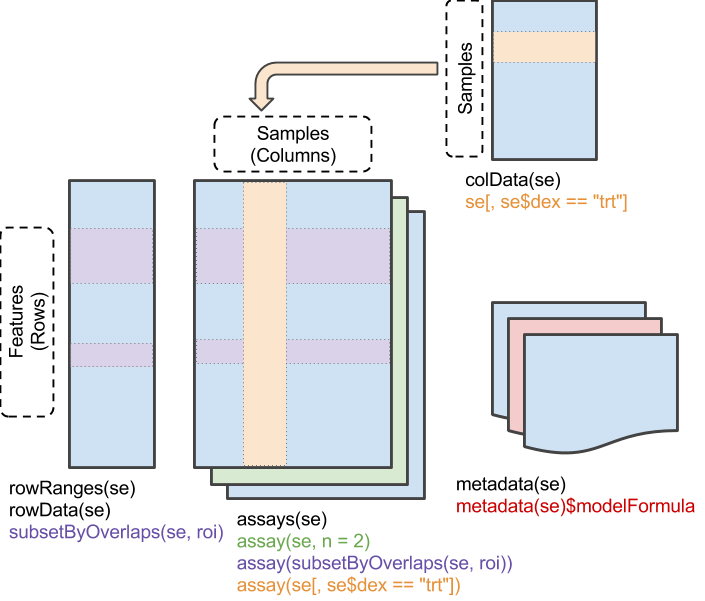
\includegraphics[width=\linewidth]{images/SummarizedExperiment.png}
    \caption{Summarised experiment data structure}
    \label{fig:sre}
\end{figure}

\section{Data preparation}
Downloaded expression data were raw counts.
To mitigate problems further down in the pipeline we performed normalization and scaling of the data.
We also visualized the effects of our normalization and scaling to assess the correctness of our steps.

\subsection{Normalisation}
In this step we performed normalisation of our data.
This was necessary, because each sample could be sequenced with different depth and we wanted to weight each sample equally.
First idea was to divide each expression entry by the median of than particular sample.
Unfortunately, this caused division by zero in some insufficiently covered samples.
Therefore we decided to divide entries by the 75th percentile of particular sample.
This should have similar effect as dividing by median and we overcome the division by zero problem in all samples.
After normalisation with percentile, we also performed logarithmic transformation of our data.
This procedure helped to reduce the strong left skew of the data and ensured that our data looked more normal.

\begin{figure}
    \centering
    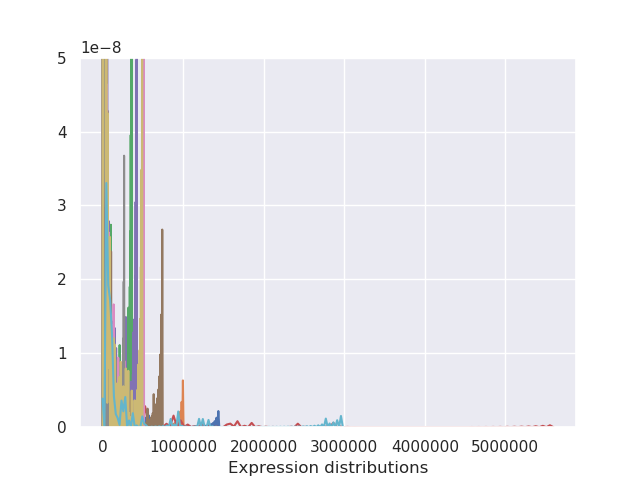
\includegraphics[width=\linewidth]{images/expr_dist.png}
    \caption{First 10 expressions before normalisation}
    \label{fig:expr_dist}
\end{figure}

\begin{figure}
    \centering
    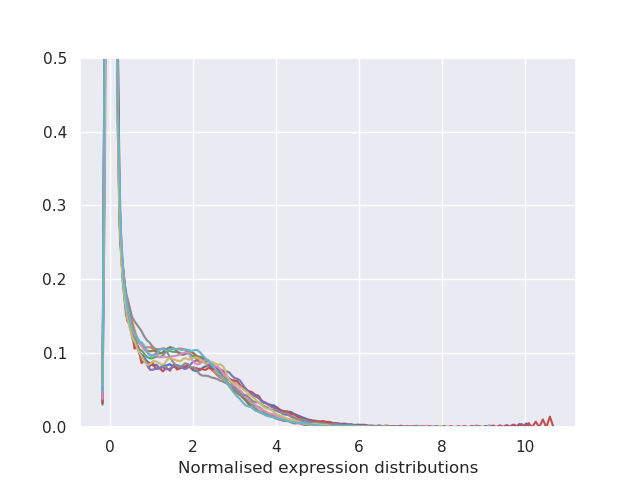
\includegraphics[width=\linewidth]{images/norm_expr_dist.png}
    \caption{First 10 expressions after normalisation}
    \label{fig:norm_expr_dist}
\end{figure}

\subsection{Scaling}
In the scaling step we adjusted each gene to have mean zero and standard deviation one.
This means, we performed row wise standardization instead column wise as in previous step.
Performed standardization was according to Equation \ref{eq:std}

\begin{equation}
    x_{ij} = \frac{x_{ij}-\bar{x_{i}}}{sd(x_{i})}
    \label{eq:std}
\end{equation}



\begin{figure}
    \centering
    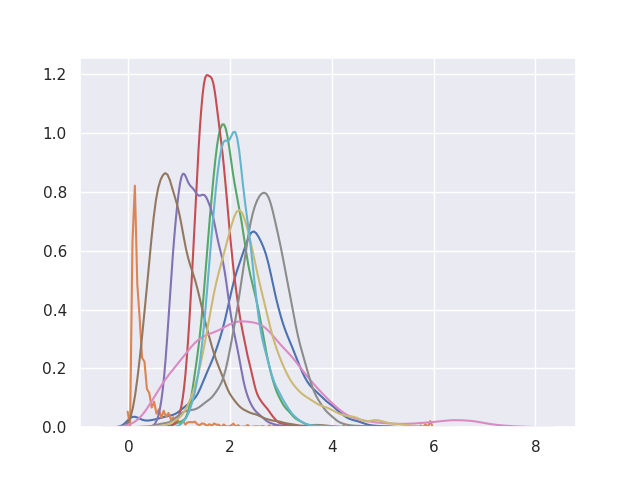
\includegraphics[width=\linewidth]{images/norm_expr_genes.png}
    \caption{Distribution of gene expression before scaling}
    \label{fig:norm_expr_genes}
\end{figure}

\begin{figure}
    \centering
    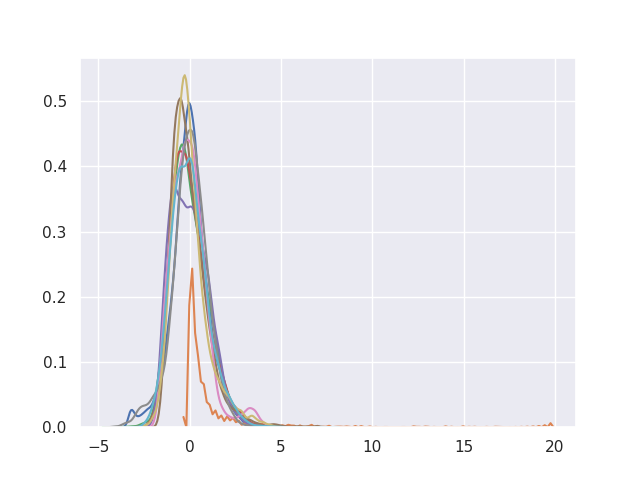
\includegraphics[width=\linewidth]{images/scaled_expr_genes.png}
    \caption{Distribution of gene expression after scaling}
    \label{fig:scaled_expr_genes}
\end{figure}


\subsection{Filtering}
In this step we calculated variation of within groups means and sorted genes descending to this value.

\subsection{PCA}
In this step we performed principal component analysis on GTEx dataset.
Then we transformed TCGA with the loading vectors from pca/

\subsection{Splitting to training, validation and testing datasets}
Because of the computational intensity of training of the neural networks we decided to validate using validation set. 
This approach can have multiple drawbacks.
% list drawbacks
To mitigate these drawbacks, we decided to perform splitting as follows.
First we removed all observations with missing value of response variable.
These would not help us to train the model.
Then we grouped remaining observations by tissue type and by cancer stage.
From each group we selected 60\% as training set, 20\% as validation set and 20\% as testing set.

\begin{figure}
    \centering
    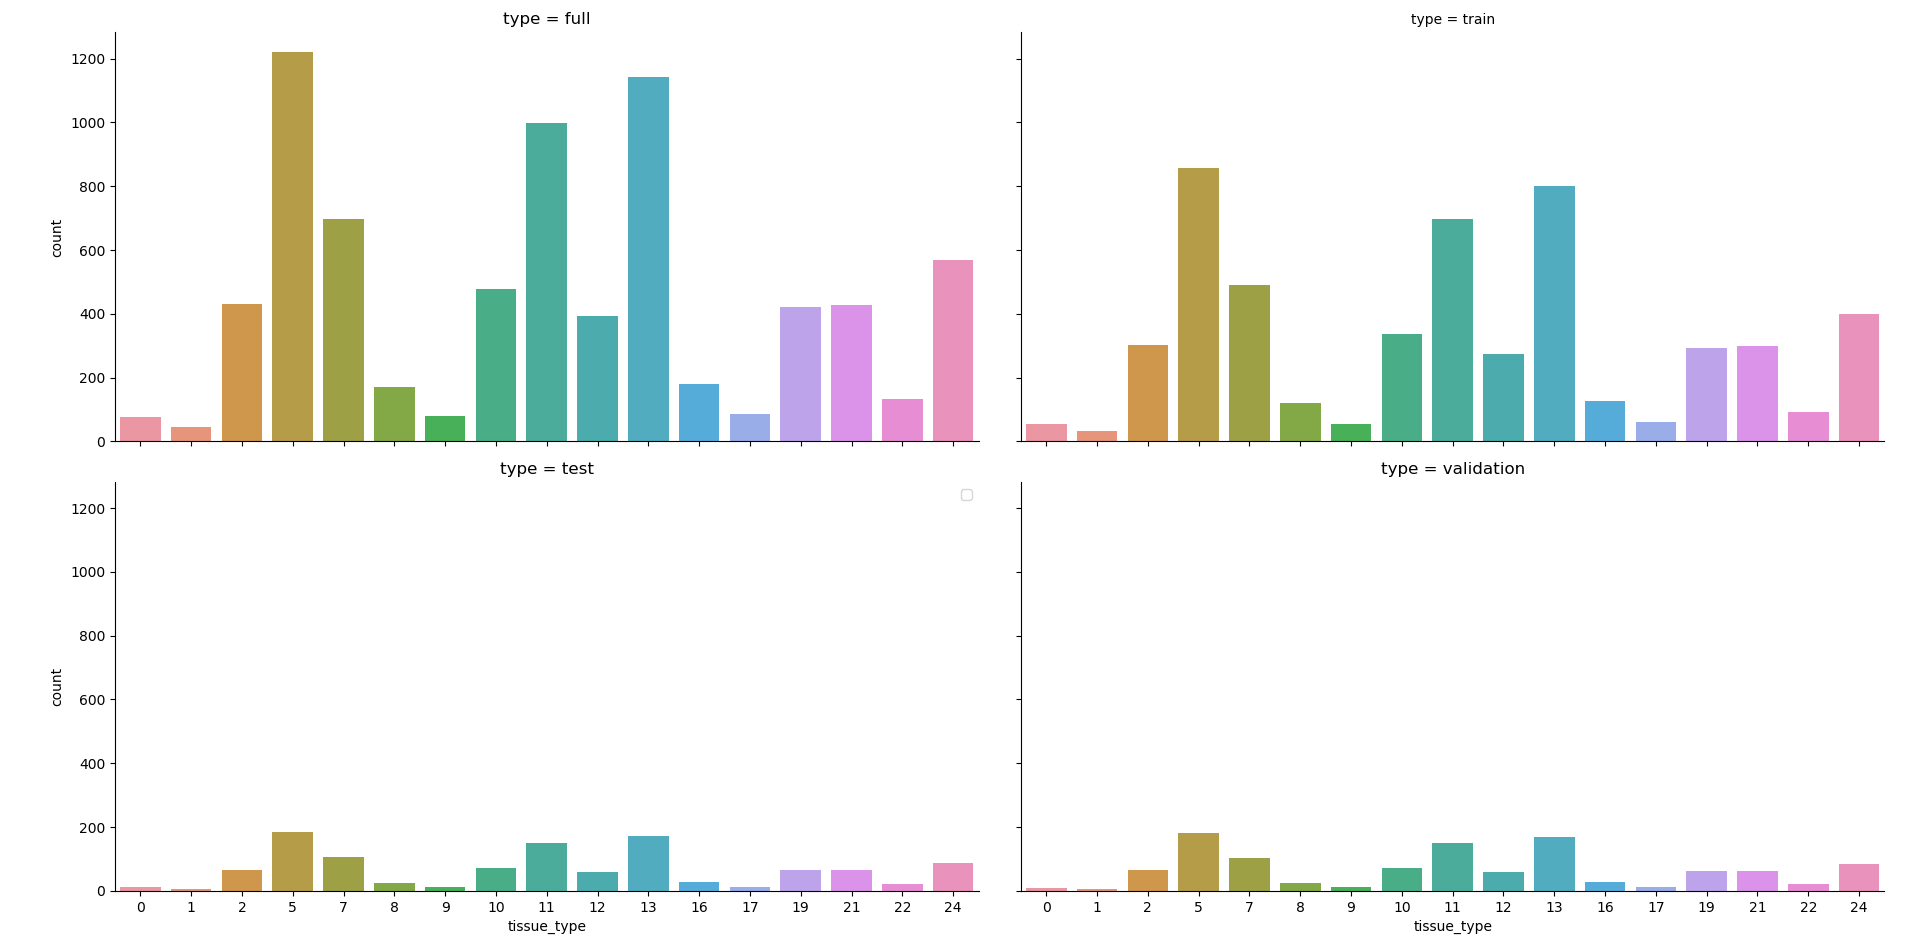
\includegraphics[width=\linewidth]{images/split_tissue.png}
    \caption{Caption}
    \label{fig:split_tissue}
\end{figure}

\begin{figure}
    \centering
    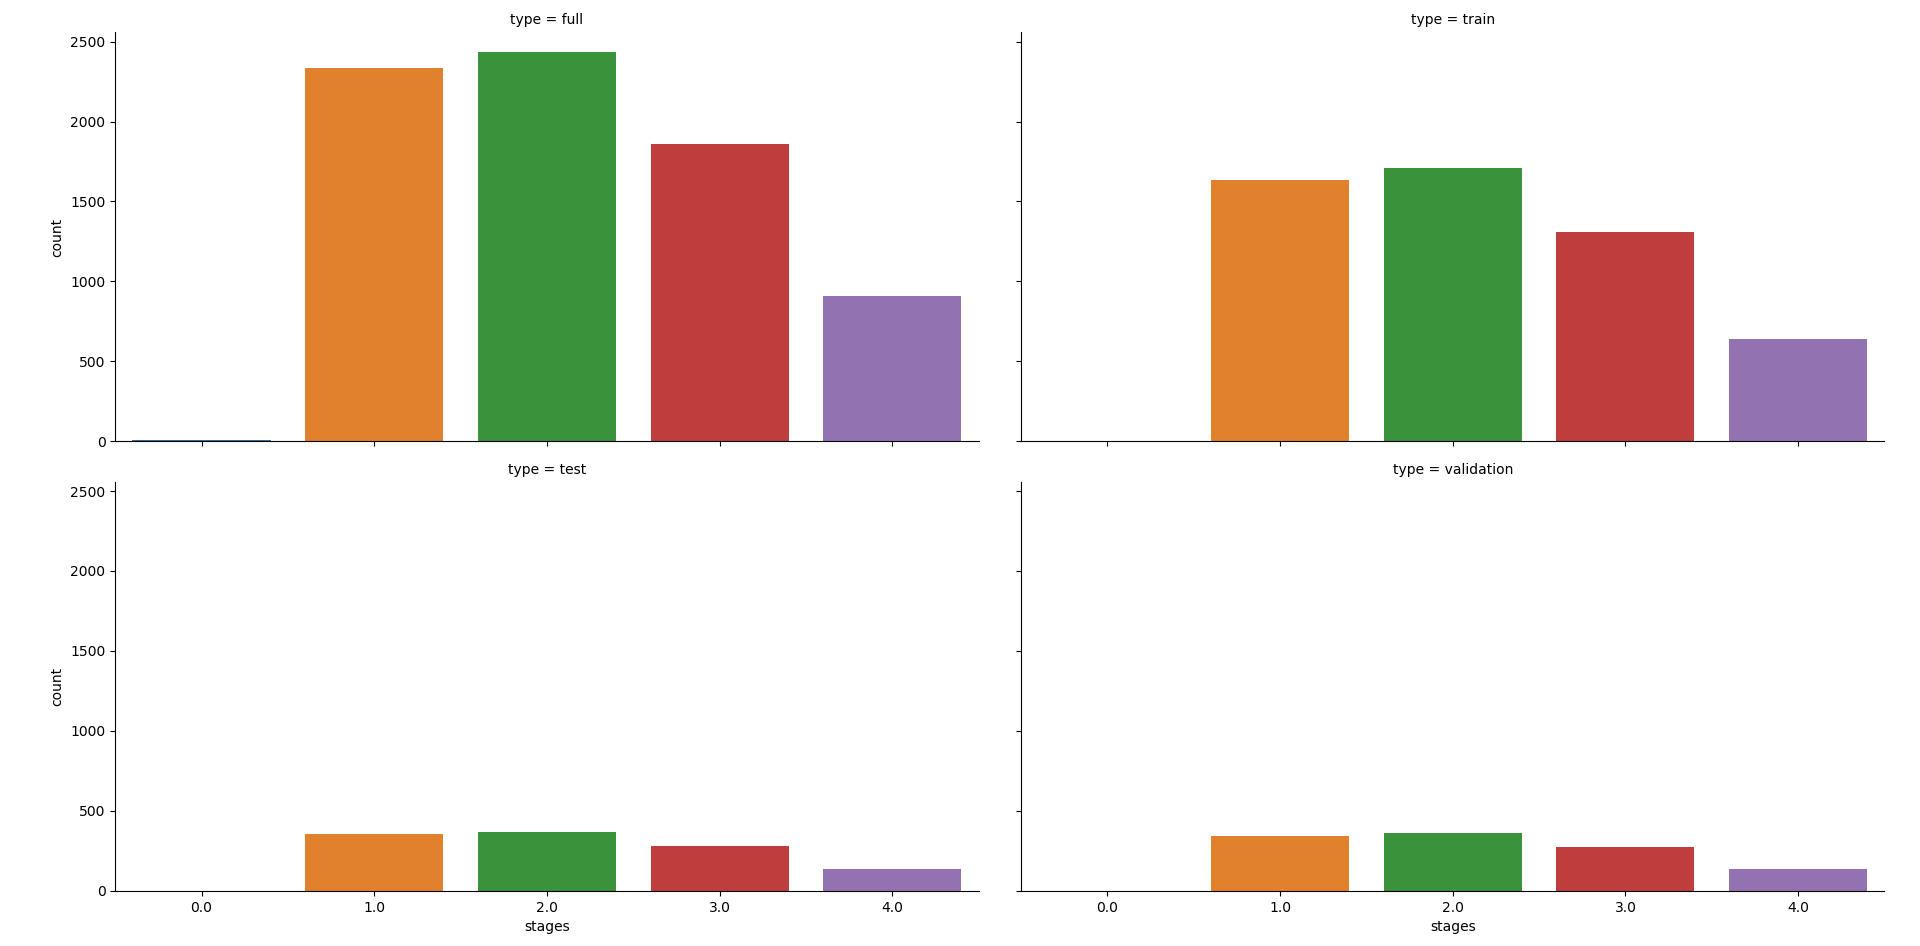
\includegraphics[width=\linewidth]{images/split_stages.png}   
    \caption{Caption}
    \label{fig:split_stages}
\end{figure}

\begin{figure}
    \centering
    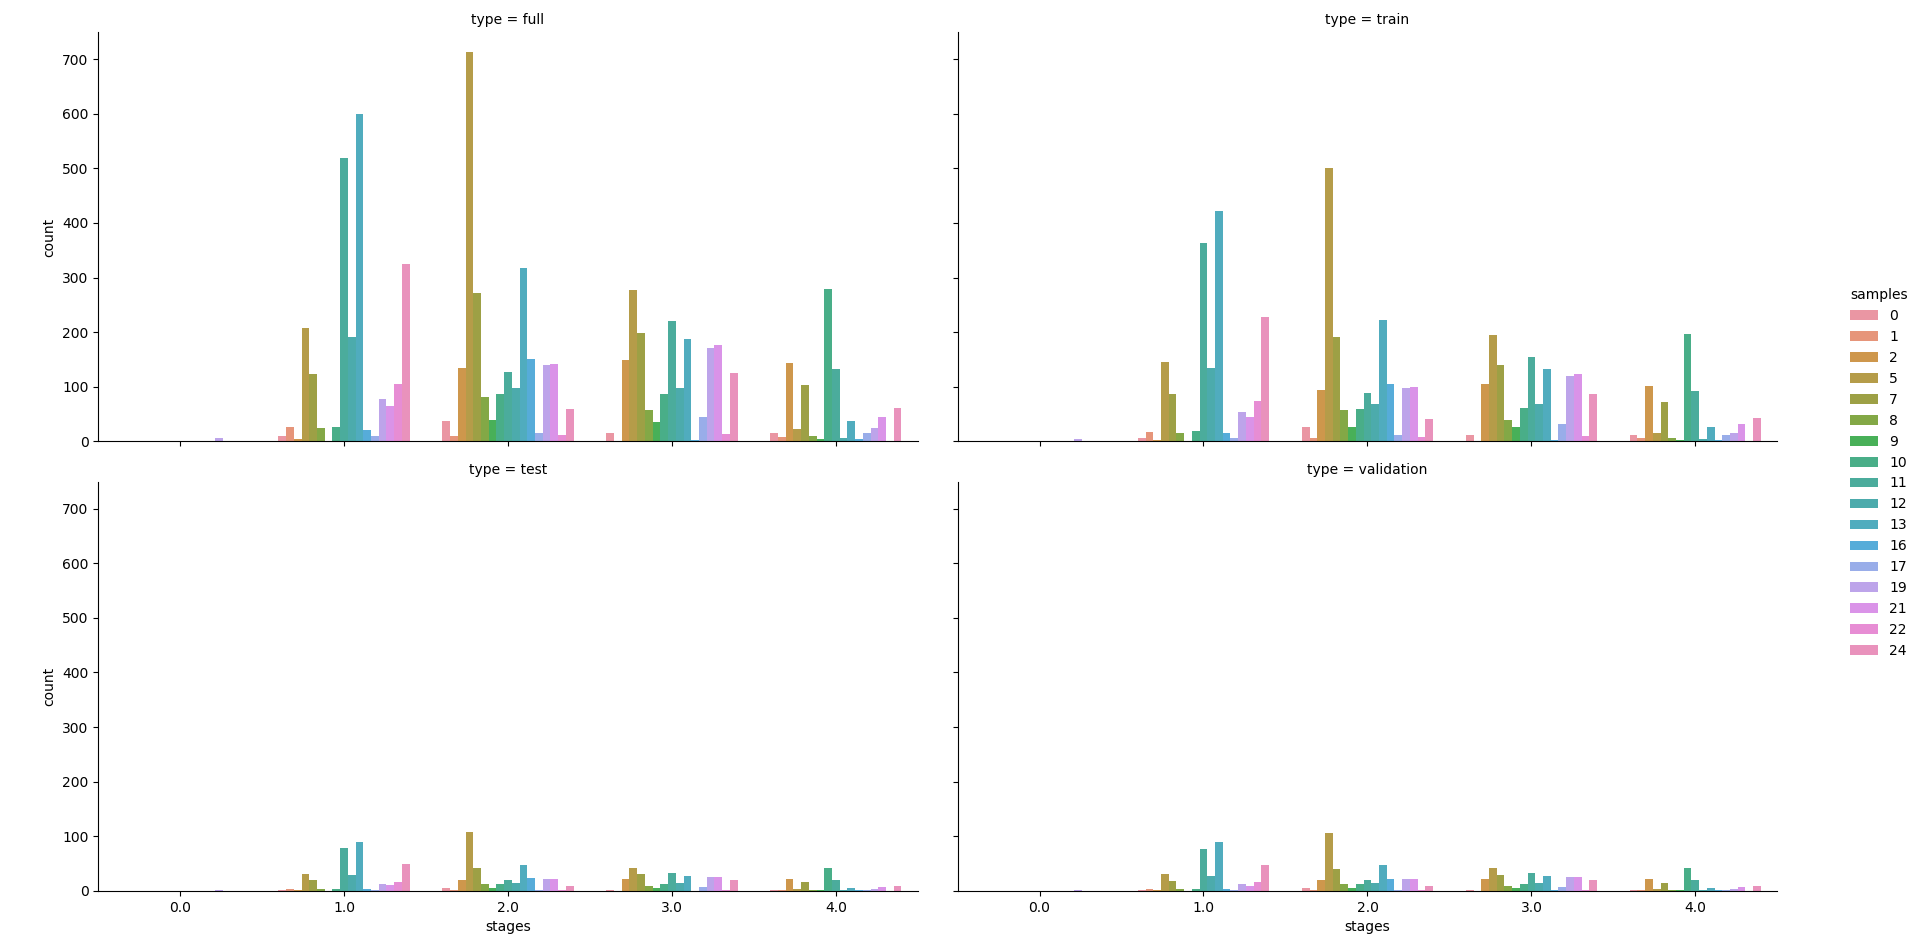
\includegraphics[width=\linewidth]{images/split_all.png}
    \caption{Caption}
    \label{fig:split_all}
\end{figure}

\section{Neural networks}
The main point of this work was to build a neural network classifier for cancer expression data.
Here we will present architecture of neural networks used.

\subsection{PyTorch library}
For building neural networks in this project we used python library PyTorch.
PyTorch library is primarily developed by Facebook's artificial inteligence research group. \cite{pytorch}
In comparison with other AI frameworks, PyTorch belongs to one of the most popular with wide support for scientific community.
It is a lower-level API directly focused on work with array expression which directly encourage the understanding of deep learning concepts.
Its lower-level approach also ensures, that the programmer has more control over the architecture.
Despite its lower-level approach it still provides automatic differentiation and backpropagation.

\subsection{Dataset object}
PyTorch provides an option to define custom dataset.
This is preferable way to use data when training the neural network, because it makes the code more clean and intuitive.
It also enables to train the model on batches which can be even shuffled.
This can make the process of training more stable and less likely to jump over some good values of parameters.
In our project we made use of these benefits of using abstract Dataset class and created custom class MyDataset extending the Dataset class.

\subsection{Feed forward neural network}
Next step was to define neural network.
We made our neural network class parametrized by the parameter architecture.
This parameter was in the format INT-...-INT, where first integer represented the size of input layer of desired neural network, last integer represented the size of output layer and all integers in the middle represented the sizes of hidden layers.
This was done using PyTorch object ModuleList to which we then added Linear layers with required parameters.
For each hidden layer we used ReLU as nonlinearity function.

\begin{figure}
    \centering
    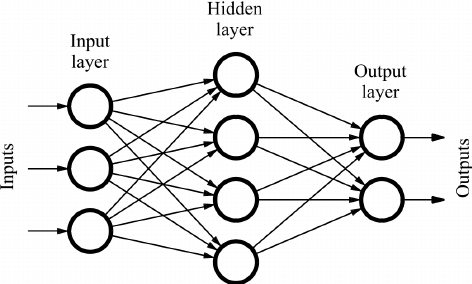
\includegraphics[width=\linewidth]{images/ff_nn.png}
    \caption{Typical neural network architecture.}
    \label{fig:ff_nn}
\end{figure}

\subsection{Pathways neural network}
In this architecture we wanted to incorporate additional information about the genes into the neural network.
For this we used KEGG data mentioned in Subsection \ref{subsec:kegg}.
First layer in the pathways neural network was our custom layer Pathways.
This layer represented membership of a gene to a particular biochemical pathway.
This was done using the binary matrix where rows represented genes and columns represented pathways.
Our custom layer then performed entrywise matrix multiplication between binary matrix and weights.
This effectively set majority of the connections to zero and the remaining connections were the one representing membership of the gene to a pathway.
This new matrix was then used for transition between input layer to the first hidden layer.
From the first hidden layer to the output layer we used Linear layers similarly to the Feed forward neural network.

\subsection{Training and regularization of the neural networks}
During the training we loaded training observations to out custom dataset class.
This class was then passed to the built in DataLoader class which allowed us to train in shuffled batches.
We also programmed this training procedure to be able to use graphical processing unit (GPU) for better performance.
As an optimized we used Adam - adaptive moment estimation \cite{kingma2014adam} optimizer with BCEWithLogitsLoss loss function. 
After each run through the whole training dataset we recorded the training loss, training accuracy, validation loss and validation accuracy.
We also stored a pickled python object of the model after each epoch.
The idea here was to perform a form of regularization, where we would choose the model with lowest validation error.
Together with this regularization, we also used dropout regularization.
Furthermore, we also tried L2 regularization. 
To estimate the hyperparameter which should be used by L2 regularization, we ran through multiple options.
The validation error using the L2 regularization can be found in the Figure \ref{}.
% add figure
Unfortunatelly, L2 regularization did not improve our accuracy over the model with just dropout, therefore we decided not to use it.


